\documentclass[journal]{new-aiaa}
%\documentclass{ahs}
%\usepackage[dvips]{graphicx}
\usepackage{graphicx}
%\usepackage{amsmath}
%\usepackage{array}
%\usepackage{latexsym}
%\usepackage{cite}
\usepackage{hyperref}
\usepackage[T1]{fontenc}
\usepackage{lmodern}
%\setmainfont[Mapping=tex-text, Color=textcolor]{CMU Serif}
%\usepackage{fancyvrb}
%\usepackage{dcolumn}
% more text vertically
%\addtolength{\textheight}{0.5in}
%\addtolength{\topmargin}{-0.5in}
% more text horizontally
%\setlength{\oddsidemargin}{0.25in}
%\setlength{\evensidemargin}{0.25in}
%\addtolength{\textwidth}{0.5in}
% more closely-positioned figures
%\renewcommand{\topfraction}{0.75}
%\renewcommand{\bottomfraction}{0.5}
%\renewcommand{\textfraction}{0.25}
%\renewcommand{\floatpagefraction}{0.75}
\usepackage{longtable,tabularx}
\setlength\LTleft{0pt}

% --------------------------------------------------------------------------

\title{Robust and Corrected Coefficients for the ROBIN Body}

\author{Blake B.~Hillier \footnote{Engineering Intern}}
\author{Mark J.~Stock \footnote{Research Scientist}}
\author{Adrin Gharakhani \footnote{President, AIAA Member}}
\affil{Applied Scientific Research, Inc.\\ Irvine, CA}

\begin{document}
\maketitle

% Technical notes have no abstract

\section*{Nomenclature}

{\renewcommand\arraystretch{1.0}
\noindent\begin{longtable*}{@{}l @{\quad=\quad} l@{}}
$(x, F(x))$  & Cartesian coordinates \\
$C_{i}$ &    $i$-th coefficient \\
$H,W$ &    height, width coefficients \\
$N$ &    elliptical power \\
$Z_{0}$ &    camber line \\
\end{longtable*}}

% --------------------------------------------------------------------------

\section{Introduction}
The ROBIN body is a VTOL fuselage shape \cite{nasa87762,mineckgorton,nasa80051,nasa1999}
which is defined by the intersection of multiple sets of analytic equations.
While the shape is used frequently in rotorcraft aerodynamics research, the coefficients,
where published, do not reliably produce the desired geometry.
While subsequent authors have presented corrections \cite{nasa87762,mineckgorton},
none have reported all that are required to generate the correct shape.
This technical note serves as a notice of correct and clarified coefficients suitable for automatic
calculation. It also provides a link to a public repository
for a program using those coefficients which generates the correct shape \cite{robinsurfmesh}.

% --------------------------------------------------------------------------

\section{Proposed changes}
In its most common form, the superellipse function used to define the ROBIN body is:
\begin{equation}
   y=r\sin(\theta) \quad z=r\cos(\theta)+Z0
\end{equation} 
where \begin{equation}
  r=\left(\frac{\left(\frac{HW}{4}\right)^{N}}{\left(\frac{H}{2}\sin(\theta)\right)^{N}+\left(\frac{W}{2}\cos(\theta)\right)^{N}}\right)^{\frac{1}{N}} \quad \theta\in[0,2\pi].
\end{equation}
$H, \ W, \ N$, and $Z0$ are all calculated from
\begin{equation}
  F\left(x\right) = C_{6}+C_{7}\left[C_{1}+C_{2}\left(\frac{x+C_{3}}{C_{4}}\right)^{C_{5}}\right]^{\frac{1}{C_{8}}}
\end{equation}
with their appropriate parameters listed in Tables 1 and 2. The current coefficients result in incorrect values for $F\left(x\right)$ which prevent obtaining the correct values for $r, \ y,$ and $z$. In order to facilitate correct computation of the shape, certain changes to the
widely-published coefficients had to be made.
Tables 1 and 2 present the complete and corrected set of coefficients with changes in bold.
The changes fall into several categories, summarized below.
\begin{itemize}
\item Denominators $C_{4}$ in the front section of both the fuselage and pylon had the wrong sign
and created incorrect results.
Figure \ref{badc4} shows both original and updated shapes.
\begin{figure} \begin{centering}
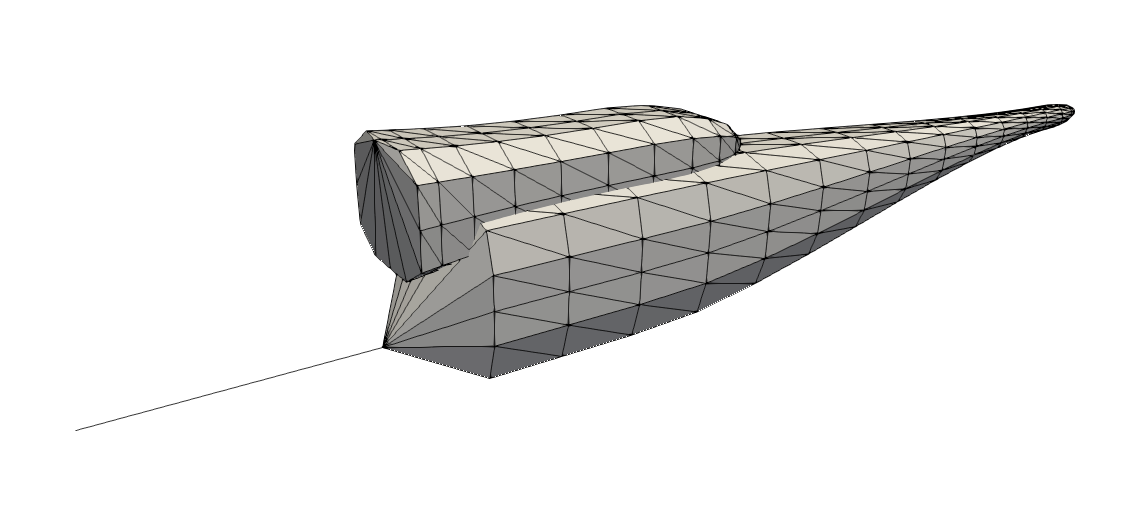
\includegraphics[width=3.0in]{img_badc4.png}
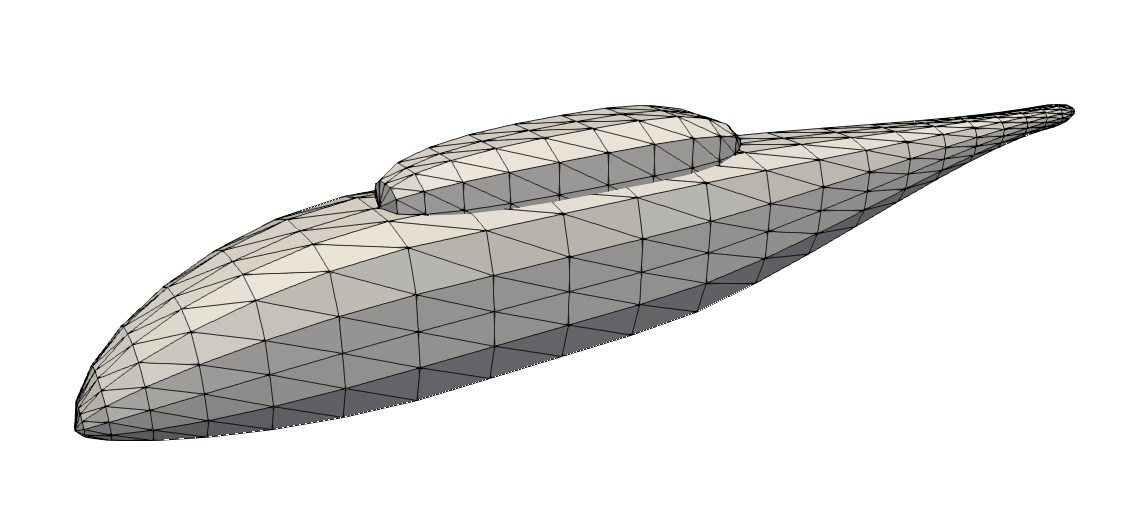
\includegraphics[width=3.0in]{img_good.png}
%\vspace{0.1in}
\caption{Shape using original formula with positive 4th coefficient, shape using correct sign.}
\label{badc4}
\end{centering}\end{figure}%
\item The denominator in the outermost exponent ($C_{8}$) was changed from 0 to 1 to prevent the evaluation from returning NaN or Inf.
This change was made where $C_{7}=0$, i.e., situations where the exponential term does not contribute to the final value.
This was pointed out by Phelps \& Berry \cite{nasa87762}.
\item Similarly, $C_{4}$ was changed from 0 to 1 to prevent division by zero, because
where $C_{2}=C_{5}=0$, there is no need to evaluate the term in the parenthesis.
\item Parameters in $C_{1}$ were often multiplied by 0 in $C_{7}$ where they were intended as the resulting values.
These single-valued parameters are more clear when they appear as the outermost constant $C_{6}$.
\item Some obvious typographic errors ($Z_0$ in the second body segment and $N$ on the pylon aft)
in the original \cite{nasa80051} were caught by later authors \cite{nasa87762,mineckgorton}, but no author caught both.
\item Components guiding the shape of the pylon ($C_{7}$) differ between earlier and later works.
We have chosen to use values from Mineck and Gorton (2000) \cite{mineckgorton} because the shape of the generated 
pylon matches the photos and drawings from earlier papers more closely \cite{nasa80051,nasa87762} than the original coefficients.
Figure \ref{badpylon} shows both original ($C_{7,H} = 0.2$, $C_{7,W} = 0.172$) and
updated ($C_{7,H} = 0.145$, $C_{7,W} = 0.166$) pylon shapes.
\begin{figure} \begin{centering}
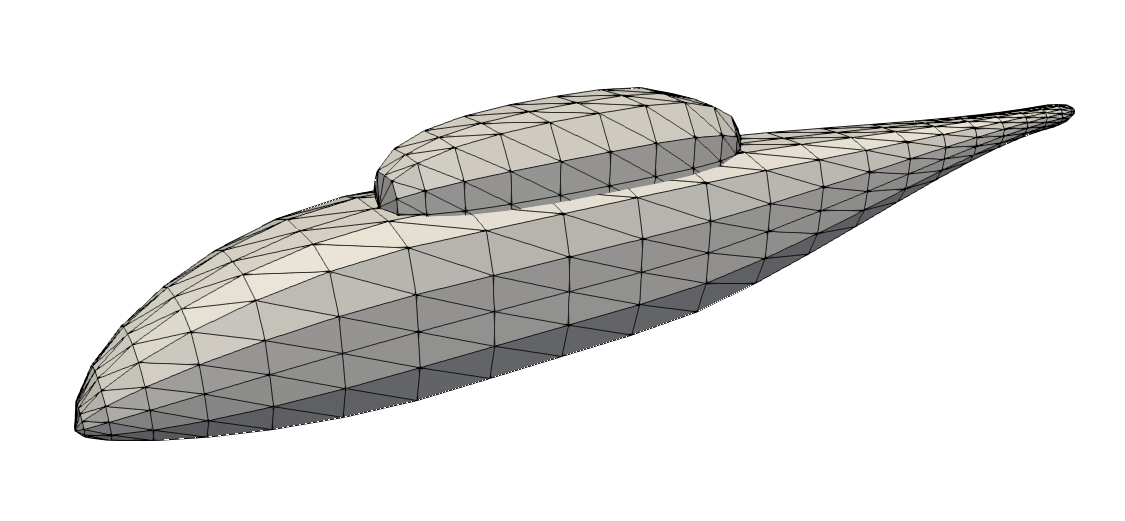
\includegraphics[width=3.0in]{img_badpylon.png}
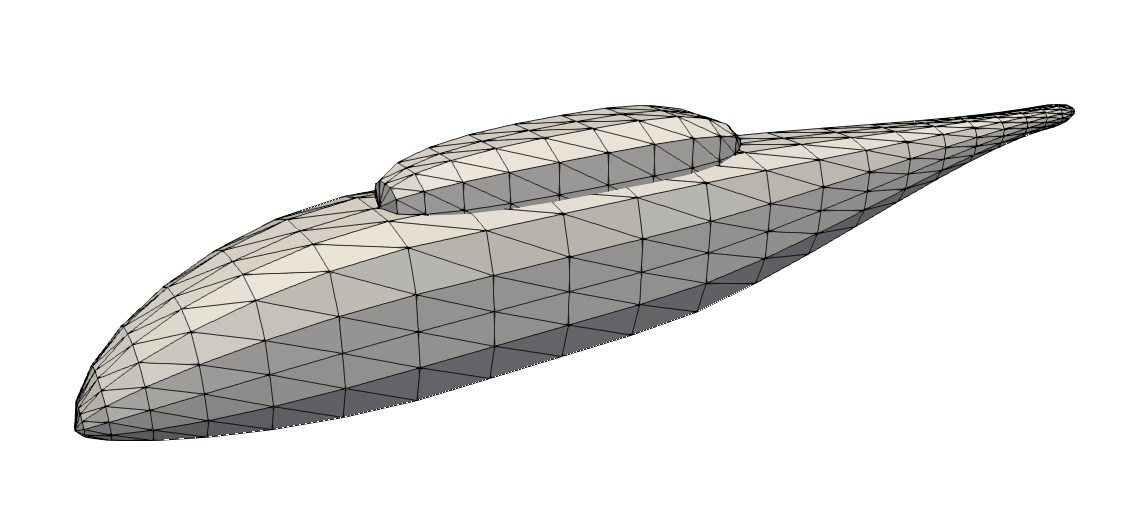
\includegraphics[width=3.0in]{img_good.png}
%\vspace{0.1in}
\caption{Pylon using original coefficients, pylon from Mineck and Gorton (2000) \cite{mineckgorton}.}
\label{badpylon}
\end{centering}\end{figure}%
\end{itemize}
\begin{table}[ht]
\caption{Coefficients for the fuselage; changes are in \textbf{bold}}
\centering
\begin{tabular}{cccccccccc}
Function & x & $C_{1}$ & $C_{2}$ & $C_{3}$ & $C_{4}$ & $C_{5}$ & $C_{6}$ & $C_{7}$ & $C_{8}$ \\
\hline
H          & [0.0, 0.4]  & 1.0 & -1.0 & -0.4 & \textbf{-0.4} & 1.8 & 0.0    & 0.25 & 1.8 \\
W          &             & 1.0 & -1.0 & -0.4 & \textbf{-0.4} & 2.0 & 0.0    & 0.25 & 2.0 \\
$Z_{0}$ &                & 1.0 & -1.0 & -0.4 & \textbf{-0.4} & 1.8 & -0.08 & 0.08 & 1.8 \\
N           &            & 2.0 & 3.0  & 0.0  &              0.4  & 1.0 & 0.0    & 1.0   & 1.0 \\
\hline
H          & [0.4, 0.8]  & \textbf{0.0} & 0.0 & 0.0 & \textbf{1.0} & 0.0 & \textbf{0.25} & 0.0 & \textbf{1.0} \\
W          &             & \textbf{0.0} & 0.0 & 0.0 & \textbf{1.0} & 0.0 & \textbf{0.25} & 0.0 & \textbf{1.0} \\
$Z_{0}$ &                & \textbf{0.0} & 0.0 & 0.0 & \textbf{1.0} & 0.0 & 0.0               & 0.0 & \textbf{1.0} \\
N           &            & \textbf{0.0} & 0.0 & 0.0 & \textbf{1.0} & 0.0 & \textbf{5.0}   & 0.0 & \textbf{1.0} \\
\hline
H          & [0.8, 1.9]  & 1.0 & -1.0 & -0.8 & 1.1 & 1.5 & 0.05 & 0.2 & 0.6 \\
W          &             & 1.0 & -1.0 & -0.8 & 1.1 & 1.5 & 0.05 & 0.2 & 0.6 \\
$Z_{0}$ &                & 1.0 & -1.0 & -0.8 & 1.1 & 1.5 & 0.04 & -0.04 & 0.6 \\
N           &            & 5.0 & -3.0 & -0.8 & 1.1 & 1.0 & 0.0 & \textbf{1.0} & \textbf{1.0} \\
\hline
H          & [1.9, 2.0]  & 1.0 & -1.0 & -1.9 & 0.1 & 2.0 & 0.0 & 0.05 & 2.0 \\
W          &             & 1.0 & -1.0 & -1.9 & 0.1 & 2.0 & 0.0 & 0.05 & 2.0 \\
$Z_{0}$ &                & \textbf{0.0} & 0.0 & 0.0 & \textbf{1.0} & 0.0 & \textbf{0.04} & 0.0 & \textbf{1.0} \\
N           &            & \textbf{0.0} & 0.0 & 0.0 & \textbf{1.0} & 0.0 & \textbf{2.0} & 0.0 & \textbf{1.0} \\
\end{tabular}
%\vspace{0.1in}
\label{fuscoeff}
\end{table}
\begin{table}[ht]
\caption{Coefficients for the pylon; changes are in \textbf{bold}}
\centering
\begin{tabular}{cccccccccc}
Function & x & $C_{1}$ & $C_{2}$ & $C_{3}$ & $C_{4}$ & $C_{5}$ & $C_{6}$ & $C_{7}$ & $C_{8}$ \\
\hline
H          & [0.4, 0.8]  & 1.0             & -1.0 & -0.8 & \textbf{-0.4} & 3.0 & 0.0                  & \textbf{0.145} & 3.0 \\
W          &                 & 1.0             & -1.0 & -0.8 & \textbf{-0.4} & 3.0 & 0.0                  & \textbf{0.166} & 3.0 \\
$Z_{0}$ &                 & \textbf{0.0} & 0.0  & 0.0  & \textbf{1.0}  & 0.0  & \textbf{0.125} & 0.0                 & \textbf{1.0} \\
N           &                 & \textbf{0.0} & 0.0  & 0.0  & \textbf{1.0}  & 0.0  & \textbf{5.0}     & 0.0                 & \textbf{1.0} \\
\hline
H          & [0.8, 1.018]  & 1.0             & -1.0 & -0.8 & 0.218         & 2.0 & 0.0                 & \textbf{0.145} & 2.0 \\
W          &                     & 1.0             & -1.0 & -0.8 & 0.218         & 2.0 & 0.0                 & \textbf{0.166} & 2.0 \\
$Z_{0}$ &                     & 1.0             & -1.0 & -0.8 & 1.1             & 1.5 & 0.065             & 0.06               & 0.6 \\
N           &                     & \textbf{0.0} & 0.0  & 0.0  & \textbf{1.0} & 0.0 & \textbf{5.0}     & 0.0                 & \textbf{1.0} \\
\end{tabular}
%\vspace{0.1in}
\label{pycoeff}
\end{table}

Code using these new coefficients can be found at the following Github link:
\url{https://github.com/Applied-Scientific-Research/robin-surface-mesh} 
\cite{robinsurfmesh}
and is able to generate a triangular mesh with customizable inputs of the number
of nodes across the length of the fuselage and pylon, 
and the number of nodes on the circumference of the fuselage and pylon.

% --------------------------------------------------------------------------
%\bibliographystyle{abbrv}
\bibliography{robinbib}
%--------------------------------------------------------------------------- 

\end{document}
